\chapter{Proposta de trabalho}

Este capítulo evidencia o que será desenvolvido, ou seja, a proposta inicial do software PGTBL.

Recapitulando, o objetivo do projeto é a automatização do metodologia ativa de aprendizagem baseada em equipe ou TBL, essa metodologia é uma estratégia de ensino colaborativa que se concentra em um ciclo de quatro passos:

\begin{enumerate}
  \item \textbf{Preparação}: Basicamente o professor irá disponibilizar de artigos e livros para estudo que será a preparação para as avaliações.
  \item \textbf{Avaliação em classe}: A primeira avaliação é individual e a segunda em grupo para testar o conhecimento adquirido na preparação e o trabalho em equipe respectivamente.
  \item \textbf{Pequeno projeto centrado na aplicação}: Aplicar todo o conhecimento adquirido em um contexto real no tópico proposto.
  \item \textbf{Avaliação em pares}: Avaliar o desempenho de cada membro da equipe.
\end{enumerate}

\section{Finalidade do software}

A finalidade do software é que a aplicação do TBL se torne algo mais fácil, constante e automatizado, tornando o processo mais prazeroso, tanto para o aluno quanto para o professor. A ideia do sistema é ter um design atrativo e será responsável por todo o processo do TBL desde a preparação até as avaliações e fechamento da disciplina.

\section{Descrição dos usuários}

Temos no total três tipos de usuários:

O usuário professor é aquele que busca melhorar o ensino e a forma de avaliação das escolas, ele tem como responsabilidade gerenciar as disciplinas e alunos usando o sistema. O professor também é responsável por criar e gerenciar as listas de exercício e avaliações.

O usuário monitor são alunos ou professores que buscam ajudar na aplicação do TBL dentro da plataforma. Tem como responsabilidade criar e gerenciar questões da lista de exercícios, arquivos da disciplina e das sessões de TBL e tirar dúvidas.

Já o usuário aluno são aqueles que querem aprender e se preparar para o mercado de trabalho de forma colaborativa e não competitiva. Tem como responsabilidade realizar todas as atividades relacionadas ao TBL.

\section{Visão geral do produto}

Este sistema tem como objetivo inovar a forma como as escolas/universidades ensinam seus alunos através do TBL, fazendo com que eles tenham uma preparação mais adequada para atuar no mercado, tendo a participação ativa dos alunos e aprimorando seu trabalho em equipe.

\subsection{Recursos do produto (Requisitos funcionais ou Épicos)}

\begin{table}[h!]
  \centering
  \caption{Requisitos Funcionais ou Épicos do produto}
  \label{tab:21}
  \begin{tabular}{@{}ll@{}}
    \toprule
    \textbf{Recurso}                                                           & \textbf{Descrição}
    \\ \midrule
    \begin{tabular}[c]{@{}l@{}}Administrar Disciplinas\\ e alunos\end{tabular} & \begin{tabular}[c]{@{}l@{}}O professor
      pode adicionar, remover, criar e editar disciplinas\\ e turmas e disponibilizar a senha de acesso a elas para os
  alu-\\ nos entrarem, além de poder remover ou adicionar estudantes\\ na turma e gerenciar suas notas.\end{tabular}
  \\ \midrule
  Criar conta                                                                & \begin{tabular}[c]{@{}l@{}}O professor e
    os alunos pode criar sua contas no sistema,\\ apenas passando seus dados pessoais como nome, email,\\ senha, e
  usuário\end{tabular}
  \\ \midrule
  \begin{tabular}[c]{@{}l@{}}Gerenciar dados\\ pessoais\end{tabular}         & \begin{tabular}[c]{@{}l@{}}O usuário
poderá editar sua senha e dados pessoais do\\ usuário conforme necessário.\end{tabular}
\\ \midrule
\begin{tabular}[c]{@{}l@{}}Funcionalidades do\\ TBL\end{tabular}           & \begin{tabular}[c]{@{}l@{}}Funcionalidades
  relacionadas às fases de preparação, garantia\\ de preparo ou RAT, iRAT, gRAT e apelações, Aplicação de\\ conceitos e
  avaliação em pares\end{tabular}                                                                                   \\
  \midrule
  Relatório                                                                  & \begin{tabular}[c]{@{}l@{}}O professor
    terá um dashboard com relatórios do desempenho\\ dos alunos em cada questão da avaliação, tendo um feedback\\ para o
  que ele deve focar mais nas aulas.\end{tabular}
  \\ \midrule
  Gamificação                                                         & \begin{tabular}[c]{@{}l@{}}Terá também um
    rank de grupos, na qual o primeiro colocado\\ ficará exposto no Hall da Fama que será visto por novos alunos\\ dos
    próximos semestres, não há rank individual porque o obje-\\ tivo não é a competição e sim a
  colaboração.\end{tabular} \\ \bottomrule
  \end{tabular}
\end{table}

\subsection{Restrições}

A proposta do serviço ofertado, envolve a utilização de certos recursos que necessitam de um navegador. De modo que tais recursos implicam em certas limitações do produto, estas limitações seriam:

\begin{itemize}
  \item O usuário deve dispor de um provedor de internet;
  \item O usuário deve dispor de um navegador;
\end{itemize}

\section{Requisitos de qualidade (Não funcionais ou Enables)}

\begin{itemize}
  \item \textbf{Sistema}: O sistema deve seguir a arquitetura MVT definida no documento de arquitetura e as ferramentas de desenvolvimento será o Python (versão 3.5) e o framework Django (versão 2.0) tendo atualização constante.
  \item \textbf{Suportabilidade}: O sistema poderá ser acessado em computadores pessoais - notebook, desktop – utilizando-se de um serviço de internet. Sendo uma aplicação Web compatível com os principais sistemas operacionais (Linux, Mac, Windows), acessada através do navegador Google Chrome e/ou Firefox de um dispositivo móvel ou fixo.
  \item \textbf{Qualidade}: O sistema deve seguir uma folha de estilo a ponto de o código ser legível e de fácil manutenção, tendo como base boas práticas de programação, o sistema deve ter baixo acoplamento e alta coesão além de ser modularizado focando na flexibilidade e manutenção do mesmo.
  \item \textbf{Usabilidade}: O sistema deve ser responsivo, adaptando-se à plataforma que o usuário estiver utilizando e o design deve ser fácil de usar e aprender.
  \item \textbf{Desempenho}: Por ser um sistema web o software necessita de uma conexão estável com a internet para seu funcionamento. A velocidade da internet tem impacto direto no desempenho da aplicação, sendo necessário uma velocidade suficiente para processar as informações e executar as funcionalidades do sistema.
  \item \textbf{Segurança}: O sistema deve apresentar uma boa percentagem de cobertura de testes automatizados, mínimo de 70\% e bastante encapsulamento de código, além de um sistema de log eficiente e ter confiabilidade.
  \item \textbf{Confiabilidade}: O sistema deve se comprometer em apresentar informações confiáveis para o usuário do sistema, entretanto dependerá diretamente dos demais usuários, uma vez que o conteúdo apresentado será de autoria destes e deve apresentar um sistema de autenticação, autorização e recuperação seguro e eficiente.
\end{itemize}

Para uma melhor visualização e rastreabilidade de requisitos não funcionais, no apêndice \ref{apendice:nfr} está o framework NFR.

\section{Alternativas e Concorrências}

Não foi encontrada nenhum site que automatiza as tarefas do Team Based Learning, apenas artigos, livros e sites ensinando como aplicar o TBL dentro das universidades e escolas usando apenas papel e caneta e algumas ferramentas de CMCs.

\begin{itemize}
  \item \href{https://aprender.unb.br/}{Moodle}: Mesmo que siga a mesma ideia do software proposto o moodle normalmente serve só para disponibilizar informações e arquivos relevantes para os alunos.
  \item \href{https://iesb.blackboard.com/}{Blackboard IESB}: Também segue a mesma ideia, mas não aplica conceitos do Team Based Learning.
\end{itemize}

\section{Ferramentas e Tecnologias}

Abaixo será listado todas as ferramentas e tecnologias que será utilizadas para a realização do projeto.

\begin{itemize}
  \item \textbf{Draw.io}: Criação de diagramas.
  \item \textbf{Google Drive}: Armazenamento e edição colaborativa dos artefatos e documentos do projeto.
  \item \textbf{Git e Github}: Controle de versão do código para um bom gerenciamento do mesmo.
  \item \textbf{Zenhub}: Permitir o gerenciamento constante das tarefas que serão realizadas durante o projeto.
  \item \textbf{Linux ubuntu}: Ambiente de desenvolvimento, homologação, produção e teste.
  \item \textbf{Whatsapp e Email}: Permite a comunicação entre os membros da equipe e os stakeholders, além da
    comunicação presencial.
  \item \textbf{Travis CI}: Ferramenta responsável por realizar a integração contínua das funcionalidades realizadas
  \item \textbf{Codacy}: Ferramenta para cobertura de testes e análise estática de código, usado para coletar métricas e
    melhorar a qualidade do código.
  \item \textbf{Docker}: Ferramentas responsáveis por criar um ambientes de desenvolvimento, teste, homologação e produção
  \item \textbf{DockerHub}: Repositório para armazenar as imagens de cada ambiente.
  \item \textbf{Python 3.5}: Linguagem de programação para a criação do software.
  \item \textbf{Django 2.0}: Framework utilizado para a criação do software.
  \item \textbf{Makefile}: Usado para facilitar a execução de scripts.
  \item \textbf{mkdocs}: Usado para criar a documentação do software.
\end{itemize}

\section{EAP, Roadmap e Canvas}

O projeto tem como base dois principais marcos definidos na tabela \ref{tab:22}, que representam entregas do produto, são eles: \textit{Release 01} e \textit{Release 02}.

\begin{table}[h!]
  \centering
  \caption{Marcos do projeto}
  \label{tab:22}
  \begin{tabular}{@{}lll@{}}
    \toprule
    \textbf{Marco}             & \textbf{Data} & \textbf{Atividade}
    \\ \midrule
    \textbf{Início do projeto} & 03/10/2017    & Começo do projeto
    \\ \midrule
    \textbf{Release 01}        & 01/08/2018    & \begin{tabular}[c]{@{}l@{}}Entrega da primeira versão funcional do
    sistema\\ com algumas funcionalidades implementadas e\\ testadas, além de sua documentação\end{tabular}           \\
    \midrule
    \textbf{Release 02}        & 01/03/2019    & \begin{tabular}[c]{@{}l@{}}Entrega do versão final do projeto com as
    funcio-\\ nalidades restantes do escopo previamente definido\\ com a utilização da abordagem ágil.\end{tabular} \\
    \bottomrule
  \end{tabular}
\end{table}

\subsection{EAP - Estrutura Analítica do Projeto}

A Estrutura Analítica do Projeto ou EAP, foi utilizada como entrada do processo fornecendo os pacotes de trabalho previamente discutidos. Esses pacotes foram então decompostos de maneira a gerar suas respectivas atividades.

A EAP se encontra no apêndice \ref{apendice:eap}

\subsection{Roadmap}

Roadmap definido na figura \ref{fig:roadmap1} e figura \ref{fig:roadmap2} é uma ferramenta muito útil para gestores de produto. Com ele é possível planejar e comunicar a visão de futuro que vc tem para o seu produto. É o cronograma da metodologia ágil.

O ROADMAP se encontra no apêndice \ref{apendice:roadmap}

\subsection{Canvas}

Canvas é um modelo visual que possibilita as pessoas de forma resumida te uma ideia do que é o projeto (canvas de projeto) e o modelo de negócio (canvas de negócio) e está localizado no apêndice \ref{apendice:canvas}.

\section{Arquitetura do Software}

O objetivo dessa seção é apresentar e detalhar a arquitetura que será utilizada na plataforma PGTBL. O desenvolvedor que
ler essa seção obterá uma visão geral de como esse software está estruturado.

\subsection{Representação Arquitetural}

O projeto será implementado utilizando o framework Django na versão 2.0. O django utiliza-se do MVT (Model-View-Template) como uma adaptação do MVC (Model-View-Controller), nas views utilizaremos as \textit{Class Based Views} para padronização do código. Esse framework fará comunicação com o banco de dados Postgresql e o servidor nginx.

\begin{figure}[H]
	\centering
  \includegraphics[keepaspectratio=true,scale=0.4]{figuras/arquitetura.eps}
  \caption[Representação Arquitetural.]{Representação Arquitetural. Fonte: Autor}
	\label{fig:arquitetura}
\end{figure}

\begin{enumerate}
  \item O web client (navegador) manda uma requisição para o web server (Nginx) com o protocolo HTTP.
  \item Os arquivos estáticos armazenados no sistema de arquivos, como CSS, JavaScript, Imagens e documentos PDF,
    podem ser processados diretamente pelo web server (Nginx).
  \item A parte dinâmica é delegada ao servidor de aplicativos WSGI (Web Server Gateway Interface) do django, no caso
    o gunicorn que é um servidor WSGI para Unix feito em python puro, ele irá converter solicitações HTTP recebidas
    do servidor em chamadas python em colaboração com o framework django que irá ter um arquivo chamado urls.py que
    diz ao nginx qual código deverá ser executado de acordo com o path e código HTTP recebido, através de proxy
    reverso será feito o redirecionamento inicial do Nginx com o servidor da aplicação, ou seja, o proxy reverso
    irá funcionar como uma ponte de ligação entre o nginx e o django através do gunicorn.
  \item Dentro do django a requisição recebida pelo web server é mapeado para uma view especifica através das urls,
    a view pede dados a modelo, a model pega os dados do banco de dados postgresql e retorna a view, esta seleciona
    o template e fornece os dados, com isso o template é preenchido e devolvido a view que devolve o template como
    resposta ao web server.
  \item O web server (nginx) retorna a resposta para o web client (navegador)
\end{enumerate}

\subsection{Pacotes Significativos do Ponto de Vista da Arquitetura}

\begin{figure}[H]
	\centering
  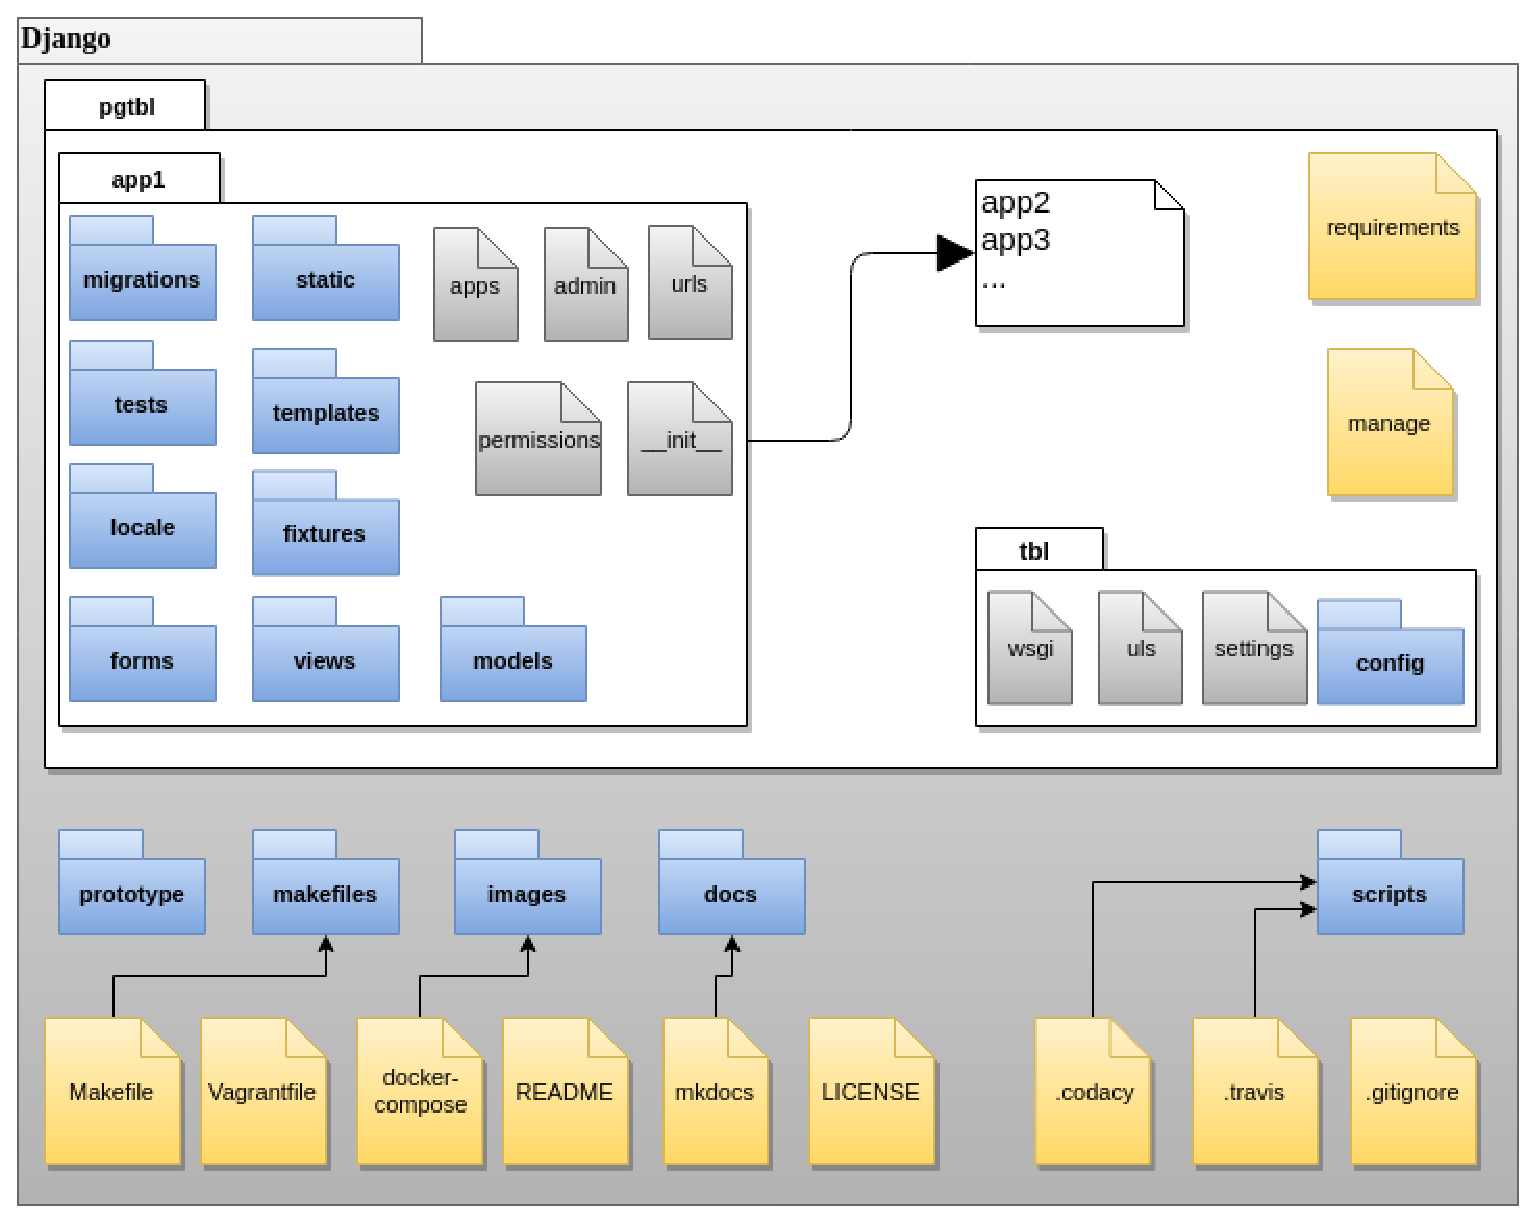
\includegraphics[keepaspectratio=true,scale=0.5]{figuras/pacotes.eps}
  \caption[Pacotes do projeto.]{Pacotes do projeto. Fonte: Autor}
	\label{fig:pacotes}
\end{figure}

\begin{itemize}
  \item Os pacotes de cada aplicação:
  \begin{itemize}
    \item \textbf{locale}: Pasta que irá ter toda a tradução do software para pt-BR.
    \item \textbf{migrations}: pasta com todas as migrações das modelos para o banco, são os SQLs.
    \item \textbf{static}: É onde fica os arquivos estáticos da aplicação (CSS, JS e IMG)
    \item \textbf{templates}: É onde fica os templates da aplicação (HTML)
    \item \textbf{tests}: contém os testes automatizados feitos no sistema.
    \item \textbf{\_\_init\_\_}: É o arquivo que define que sua pasta é um pacote python.
    \item \textbf{admin}: contém a instância da modelo que fará parte do sistema de administração do django.
    \item \textbf{app}: arquivo que contém informações da aplicação do django.
    \item \textbf{forms}: pasta que contém os campos que será inserido no formularios
    \item \textbf{models}: pasta de arquivos que faz interface com o banco de dados, é responsável por leitura,
      validação e escrita de dados no banco de dados.
    \item \textbf{permissions}: Arquivo de implementação de permissões do aplicativo.
    \item \textbf{urls}: São as rotas para ser acessada pelo navegador
    \item \textbf{views}: pasta que contém a camada lógica do sistema e a comunicação com o navegador por meio de
      rotas (Classe Based Views).
    \item \textbf{fixtures}: pasta que contém arquivos json para pré-popular o banco de dados para testes manuais
  \end{itemize}
  \item Os pacotes de configuração:
  \begin{itemize}
    \item \textbf{config}: É uma pasca que contém as configurações do software separada em arquivos.
    \item \textbf{settings}: São as configurações gerais do software importadas da pasta config.
    \item \textbf{urls}: Arquivo que terá o mapeamento de rotas de todo o projeto com todas as aplicações.
    \item \textbf{wsgi}: Arquivo usado para deploy do projeto.
  \end{itemize}
  \item Os pacotes do projeto Django:
  \begin{itemize}
    \item \textbf{manage}: Arquivo de configuração geral do django.
    \item \textbf{requirements}: Arquivos para instalar dependências da aplicação através do seguinte comando:
      pip3 install -r requirements.txt
  \end{itemize}
  \item Os pacotes gerais do projeto PGTBL:
  \begin{itemize}
    \item \textbf{Vagrantfile}: Arquivo que gerencia a máquina virtual de desenvolvimento, criado para desenvolvedores
      que queiram desenvolver em sistemas operacionais diferentes do Linux, como Windows ou Mac, precisa ter o
      Vagrant instalado.
    \item \textbf{Makefile}: Arquivo de atalhos para comandos muito usados pelos desenvolvedores.
    \item \textbf{docker-compose}: Arquivos que gerencia todos os containers da aplicação
      (deploy, homolog, production, test e desenvolvimento).
    \item \textbf{.travis}: Arquivo que gerencia a entrega continua da aplicação através da ferramenta Travis CI no github.
    \item \textbf{.codacy}: Arquivo de configuração da ferramenta de análise estática de código Codacy.
    \item \textbf{.gitignore}: Arquivo que faz o git ignorar alguns arquivos do projeto.
    \item \textbf{README}: Arquivo com um conteúdo markdown inicial do projeto.
    \item \textbf{LICENSE}: Licença do software.
    \item \textbf{mkdocs}: Arquivo que contém a configuração da documentação do software.
    \item \textbf{prototype}: Pasta com o protótipo do software.
    \item \textbf{docs}: Pasta com toda a documentação do software.
    \item \textbf{makefiles}: Pasta que contém de forma organizada comandos do Makefile.
    \item \textbf{images}: Pasta que armazena as imagens de deploy da aplicação tbl.
    \item \textbf{scripts}: Pasta com alguns scripts de integração e deploy continuo
  \end{itemize}
\end{itemize}
